%% ============================================================
%%  WCSTNet — IEEE Journal Full Paper Skeleton
%%  Wavelet CNN Squeeze-Excitation Transformer Network
%%  Target: IEEE JBHI or IEEE TNSRE
%%
%%  FIGURE MAP (ALL figures listed in order):
%%  Fig 1  — fig1_intro.pdf         (generate_intro_fig.py)
%%  Fig 2  — fig2_sensor_layout.pdf (generate_sensor_layout.py)
%%  Fig 3  — fig_pipeline_v4.pdf    (draw.io — see drawio_pipeline_guide.txt)
%%  Fig 4  — TikZ 3D CNN tensor     (inline TikZ — no external file)
%%  Fig 5  — 2.pdf                  (Max/Avg pooling illustration)
%%  Fig 6  — TikZ SE attention flow (inline TikZ — no external file)
%%  Fig 7  — 5.pdf                  (SE squeeze-excite-scale diagram)
%%  Fig 8  — 4.pdf                  (Transformer MHA + FFN block)
%%  Fig 9  — 6.pdf                  (Attention key/query saliency hook)
%%  Fig 10 — 7.pdf                  (Architecture equation overview)
%%  Fig 11 — fig_ablation_baseline.pdf / fig_comparative_bar.pdf
%%  Fig 12 — 183550.png + 183551.png (confusion matrices — window + subject)
%%  Fig 13 — fig_per_subject.pdf    (generate_paper_figs.py)
%%  Fig 14 — fig_window_ablation.pdf(generate_paper_figs.py)
%%  Fig 15 — 183552.png + 183553.png (ROC + PR curves)
%%  Fig 16 — fig_hy_staging.pdf     (generate_paper_figs.py)
%%  Fig 17 — fig_tsne.pdf           (generate_paper_figs.py)
%%  Fig 18 — fig_temporal_saliency.pdf (generate_paper_figs.py)
%%  Fig 19 — 183555.png             (Transformer attention heatmap)
%% ============================================================

\documentclass[lettersize,journal]{IEEEtran}

%% ---- Core packages ----
\usepackage{amsmath,amsfonts,amssymb}
\usepackage{algorithmic}
\usepackage{algorithm}
\usepackage{array}
\usepackage[caption=false,font=normalsize,labelfont=sf,textfont=sf]{subfig}
\usepackage{textcomp}
\usepackage{stfloats}
\usepackage{url}
\usepackage{verbatim}
\usepackage{graphicx}
\usepackage{cite}
\usepackage{booktabs}
\usepackage{multirow}
\usepackage{eqparbox}
\usepackage{xcolor}
\usepackage{hyperref}

%% ---- TikZ ----
\usepackage{tikz}
\usepackage{tikz-3dplot}
\usetikzlibrary{
    arrows.meta,
    positioning,
    shapes.geometric,
    calc,
    3d,
    matrix,
    bending
}

%% ---- 3D matrix TikZ styles (for CNN tensor figure) ----
\newbox\matrixcellbox
\tikzset{
    math center align per matrix/.style={
        nodes={
            execute at begin node={\setbox\matrixcellbox=\hbox\bgroup$},
            execute at end node={$\egroup\eqmakebox[\tikzmatrixname][c]{\copy\matrixcellbox}}
        }
    },
    3d matrix/.style={
        matrix of nodes,
        nodes in empty cells,
        math center align per matrix,
        nodes={
            draw=black!80, thick, fill=white,
            anchor=center,
            outer sep=0pt,
            inner sep=2pt,
            text height={height("\raisebox{0.2ex}{A}")},
            text depth={depth("g")},
            font=\tiny\bfseries
        },
        column sep=-\pgflinewidth,
        row sep=-\pgflinewidth,
        execute at end matrix={
            \foreach \XX in {1,...,\the\pgfmatrixcurrentcolumn}
                {\draw[thick, black!80] (\tikzmatrixname-1-\XX.north east) -- ++ (1ex,1ex);}
            \ifnum\the\pgfmatrixcurrentrow>1
                \foreach \XX in {1,...,\the\numexpr\the\pgfmatrixcurrentrow-1}
                    {\draw[thick, black!80] (\tikzmatrixname-\XX-\the\pgfmatrixcurrentcolumn.south east) -- ++ (1ex,1ex);}
            \fi
            \draw[thick, black!80] (\tikzmatrixname-1-1.north west) -- ++ (1ex,1ex) --
                  ([xshift=1ex,yshift=1ex]\tikzmatrixname-1-\the\pgfmatrixcurrentcolumn.north east) --
                  ([xshift=1ex,yshift=1ex]\tikzmatrixname-\the\pgfmatrixcurrentrow-\the\pgfmatrixcurrentcolumn.south east) --
                  (\tikzmatrixname-\the\pgfmatrixcurrentrow-\the\pgfmatrixcurrentcolumn.south east);
        }
    },
    3d matrix/.default=1ex,
    Rightarrow/.style={
        double,
        double distance=#1,
        >={Implies[bend]},
        shorten <=0.4ex
    },
    Rightarrow/.default=1ex
}

%% ---- Colours ----
\definecolor{dgreen}{RGB}{63,127,0}
\definecolor{dred}{RGB}{144,14,3}
\definecolor{wcst_blue}{RGB}{26,111,175}
\definecolor{wcst_red}{RGB}{192,57,43}
\definecolor{wcst_green}{RGB}{39,174,96}
\definecolor{wcst_purple}{RGB}{142,68,173}
\definecolor{wcst_orange}{RGB}{230,126,34}

%% ============================================================
\begin{document}

%% ===== TITLE =================================================
\title{WCSTNet: A Wavelet CNN Squeeze-Excitation Transformer Network
for Parkinson's Disease Detection from Vertical Ground Reaction
Force Signals Under Strict Subject-Level Evaluation}

\author{Subhadeep~Sasmal,~\IEEEmembership{Student Member,~IEEE},
        and Indrajit~Banerjee,~\IEEEmembership{Senior Member,~IEEE}
\thanks{Manuscript received XX Month 2025; accepted XX Month 2025.}
\thanks{S.~Chakraborty and I.~Banerjee are with the Department of
Information Technology, Indian Institute of Engineering Science and
Technology (IIEST) Shibpur, Howrah~711103, India
(e-mail: subhadeep.hyperx@gmail.com).}}

\maketitle

%% ============================================================
%%  ABSTRACT
%% ============================================================
\begin{abstract}
Parkinson's disease~(PD) is a progressive neurodegenerative disorder
whose hallmark motor symptoms—gait freezing, bradykinesia, and postural
instability—can be objectively quantified through Vertical Ground
Reaction Force~(VGRF) signals collected by pressure-insole wearables.
Although deep learning methods have achieved high reported accuracies on
the widely used PhysioNet GaitPDB benchmark, most prior works partition
data at the \emph{window level}, inadvertently allowing gait segments
from the same subject to appear in both training and test splits and
thereby inflating performance estimates.
In this paper we propose \textbf{WCSTNet} (Wavelet CNN
Squeeze-Excitation Transformer Network), a lightweight end-to-end
architecture that integrates four complementary components:
(i)~a Daubechies-4 wavelet decomposition front-end enriching each
sensor channel with multi-resolution frequency detail;
(ii)~two-stage convolutional blocks extracting local temporal patterns;
(iii)~a channel-wise Squeeze-and-Excitation attention module
recalibrating sensor importance; and
(iv)~a two-layer Multi-Head Self-Attention Transformer Encoder with
Sinusoidal Positional Encoding capturing full-stride-cycle gait phase
dependencies simultaneously.
Under strict \textit{GroupShuffleSplit} subject-level cross-validation
across 62 test subjects, WCSTNet achieves \textbf{93.9\%} window-level
accuracy, \textbf{96.8\%} subject-level accuracy (macro F1\,=\,0.960),
AUC\,=\,0.981, and Average Precision\,=\,0.994 with only
${\sim}$98\,K trainable parameters.
Transformer attention maps confirm that the model localises
diagnostically meaningful gait phases, providing clinical
interpretability absent in recurrent architectures.
\end{abstract}

\begin{IEEEkeywords}
Parkinson's disease, vertical ground reaction force, gait analysis,
Transformer encoder, squeeze-and-excitation attention, wavelet
decomposition, sinusoidal positional encoding, subject-level
evaluation, deep learning.
\end{IEEEkeywords}

%% ============================================================
%%  SECTION I — INTRODUCTION
%% ============================================================
\section{Introduction}
\label{sec:intro}

\IEEEPARstart{P}{arkinson's} disease~(PD) is the second most prevalent
neurodegenerative disorder worldwide, affecting an estimated 8--10
million people and expected to exceed 12 million by 2040 as populations
age~\cite{who2022}.
PD arises from the progressive loss of dopaminergic neurons in the
substantia nigra, producing tremor, bradykinesia, rigidity, and
postural instability that profoundly impair mobility and quality of
life~\cite{bloem2021pd}.
The Unified Parkinson's Disease Rating Scale~(UPDRS) remains the
clinical gold standard, yet relies on subjective examiner assessment
and is therefore prone to inter-rater variability and late-stage
detection~\cite{mds2003updrs}.
Consequently there is an urgent clinical need for objective,
quantifiable biomarkers that can detect and monitor PD motor
dysfunction early and unobtrusively.

%% ---- FIGURE 1: VGRF signal + evaluation protocol schematic ----
\begin{figure}[t]
\centering
% Generated by generate_intro_fig.py → figs/fig1_intro.pdf
\includegraphics[width=\columnwidth]{figs/fig1_intro.pdf}
\caption{(a)~Representative VGRF signals from sensor~L1 (posterior
heel) for a healthy control~(CO, blue) and a PD patient~(red).
PD gait exhibits reduced peak forces, prolonged stance phase, and
attenuated loading-response dynamics.
(b)~Comparison of window-level $k$-fold splitting~(prior work, left)
versus strict subject-level GroupShuffleSplit~(this work, right).
Window-level splitting leaks gait segments from the same subject into
both train and test sets, inflating reported accuracy.}
\label{fig:intro}
\end{figure}

Vertical Ground Reaction Force~(VGRF) signals, acquired via
pressure-sensitive insoles at 100\,Hz, encode plantar loading
dynamics: the characteristic double-peak of heel strike and push-off,
inter-foot asymmetry, cadence variability, and stride duration~%
\cite{alharthi2021}.
As illustrated in Fig.\,\ref{fig:intro}(a), healthy gait exhibits
sharp, well-defined loading peaks while PD gait is distinguished by
reduced force magnitudes, widened stance phases, and inter-stride
variability—manifestations of bradykinesia and impaired motor
planning~\cite{yuan2025mscaf}.

Early computational approaches relied on hand-crafted
spatiotemporal features and classical classifiers~%
\cite{alam2017vgrf,ertugrul2016lbp,prabhu2020}.
Deep learning replaced explicit feature engineering: El~Maachi
et~al.~\cite{maachi2020convnet} showed a deep 1D-ConvNet surpasses
machine-learning pipelines; Xia et~al.~\cite{xia2020dcalstm} combined
CNN and LSTM into a dual-modal architecture; and Liu et~al.~%
\cite{liu2021dualbranch} extended this to a dual-branch CNN-BiLSTM
framework.
Attention-based methods brought further gains:
Nguyen et~al.~\cite{nguyen2022transformer} applied a temporal
Transformer to 1D gait signals, and Naimi et~al.~\cite{naimi2023hct}
proposed a hybrid ConvNet-Transformer.
Graph Neural Network~(GNN) approaches explicitly model the spatial
topology of plantar sensors~\cite{zhong2022rfdgad, wang2023astdgnn,
wang2026msadgnn, wang2025gld2gnn}.
MSCAF-Gait~\cite{yuan2025mscaf} achieved 99.61\% accuracy through
multi-scale cross-attention fusion.

Despite these advances, two critical gaps persist.
\textbf{First}, the dominant experimental protocol applies $k$-fold
or sliding-window cross-validation to a pooled window dataset,
inevitably placing windows from the same subject in both train and
test—as shown in Fig.\,\ref{fig:intro}(b).
This constitutes data leakage and inflates estimates relative to true
generalisation to unseen patients.
\textbf{Second}, BiLSTM-based models process gait tokens
\emph{sequentially}: early heel-strike tokens must survive many
hidden-state transitions before contributing to classification.
Transformer self-attention resolves this by computing direct pairwise
interactions among all 47 gait tokens simultaneously, and Sinusoidal
Positional Encoding~(SinPE) additionally encodes \emph{where} in
the gait cycle each token resides.

The primary contributions of this paper are:
\begin{itemize}
    \item \textbf{WCSTNet architecture:} A novel CNN-SE-Transformer
    pipeline with Daubechies-4 wavelet multi-resolution input
    enrichment, Squeeze-and-Excitation channel recalibration,
    and a two-layer pre-norm Transformer Encoder with SinPE,
    achieving ${\sim}$98\,K parameters.
    \item \textbf{Rigorous evaluation:} Strict subject-level
    GroupShuffleSplit ensuring zero subject overlap across 62 test
    subjects—eliminating the data leakage endemic in prior work.
    \item \textbf{Confidence-weighted majority vote:} Subject-level
    diagnosis from per-window predictions, weighting confident
    windows more heavily.
    \item \textbf{Clinical interpretability:} Transformer attention
    maps revealing focus on diagnostically meaningful gait phases
    (terminal stance, pre-swing).
\end{itemize}

The remainder of this paper is organised as follows.
Section~\ref{sec:related} reviews related work.
Section~\ref{sec:method} describes dataset, preprocessing, WCSTNet
architecture, and evaluation protocol.
Section~\ref{sec:results} presents quantitative results.
Section~\ref{sec:discussion} discusses findings, limitations, and
clinical implications.
Section~\ref{sec:conclusion} concludes the paper.

%% ============================================================
%%  SECTION II — RELATED WORK
%% ============================================================
\section{Related Work}
\label{sec:related}

\subsection{Traditional Machine Learning on VGRF}
Early PD gait detection extracted hand-crafted features—temporal
stride parameters, frequency-domain spectral ratios, and statistical
moments—before training SVMs, Bayes classifiers, and random
forests~\cite{alam2017vgrf,ertugrul2016lbp,prabhu2020,
abdulhay2018,balaji2021}.
While interpretable, these methods are limited by manual feature
engineering and reduced performance under inter-subject variability.

\subsection{CNN and Recurrent Deep Learning}
CNN-based end-to-end learning overcame hand-crafting limitations~%
\cite{maachi2020convnet}.
Combining CNNs with recurrent layers provided complementary spatial
and temporal modelling: DCALSTM~\cite{xia2020dcalstm} processes the
left and right foot separately; a dual-branch CNN-BiLSTM~%
\cite{liu2021dualbranch} exploits independent and joint features.
However, recurrent architectures process data sequentially, causing
information decay over long gait windows~\cite{naimi2023hct}.

\subsection{Transformer and Attention-Based Approaches}
Transformer-based methods leverage global self-attention to capture
longer temporal dependencies~\cite{nguyen2022transformer,naimi2023hct}.
MSCAF-Gait~\cite{yuan2025mscaf} achieves 99.61\% through multi-scale
convolution and cross-attention fusion on windowed VGRF data.

\subsection{Graph Neural Networks for VGRF}
GNN methods model the inherent topological structure of plantar sensors
as a directed graph~\cite{zhong2022rfdgad,wang2023astdgnn}.
MS-ADGNN~\cite{wang2026msadgnn} builds a three-scale directed graph
with a dual-stream~(original + differential) framework.
GLD\textsuperscript{2}-GNN~\cite{wang2025gld2gnn} introduces dynamic
graph learning.
While GNN methods are architecturally compelling, they require
hand-designed graph topology and incur higher model complexity.

\subsection{Evaluation Protocol and Data Leakage}
Most methods apply 5-fold or 10-fold cross-validation to pooled
gait-cycle windows, causing subject-level data leakage~%
\cite{wang2026msadgnn}.
Cross-dataset validation partially addresses this~%
\cite{wang2023astdgnn,wang2026msadgnn}, but is sensitive to
dataset-specific distribution shifts.
In this work we adopt strict GroupShuffleSplit subject-level
cross-validation providing the most direct measure of generalisation
to unseen patients.

%% ============================================================
%%  SECTION III — MATERIALS AND METHODS
%% ============================================================
\section{Materials and Methods}
\label{sec:method}

\subsection{Dataset}
\label{sec:dataset}

We evaluate WCSTNet on the PhysioNet Gait in Parkinson's Disease
(GaitPDB) database~\cite{physionet2000}, comprising three independently
conducted studies~\cite{yogev2005,hausdorff2007,frenkel2005}:
\textbf{Ga}~(29~PD, 18~CO, dual-task walking);
\textbf{Ju}~(29~PD, 25~CO, rhythmic auditory stimulation);
\textbf{Si}~(35~PD, 29~CO, treadmill walking).
All recordings used 16 pressure sensors (8 per foot) at 100\,Hz,
measuring VGRF in Newtons over approximately two minutes.
Table~\ref{tab:dataset} summarises the dataset.

\begin{table}[!t]
\caption{PhysioNet GaitPDB Dataset Summary}
\label{tab:dataset}
\centering
\renewcommand{\arraystretch}{1.2}
\begin{tabular}{lcccc}
\toprule
\textbf{Sub-set} & \textbf{PD} & \textbf{CO} & \textbf{Sensors} &
\textbf{Task} \\
\midrule
Ga \cite{yogev2005}      & 29 & 18 & 16 & Dual-task walk \\
Ju \cite{hausdorff2007}  & 29 & 25 & 16 & Auditory stim. \\
Si \cite{frenkel2005}    & 35 & 29 & 16 & Treadmill      \\
\midrule
\textbf{Total}           & \textbf{93} & \textbf{72} & & \\
\bottomrule
\end{tabular}
\end{table}

%% ---- FIGURE 2: Sensor layout ----
\begin{figure}[!t]
\centering
% Generated by generate_sensor_layout.py → figs/fig2_sensor_layout.pdf
\includegraphics[width=\columnwidth]{figs/fig2_sensor_layout.pdf}
\caption{Spatial layout of the 16 VGRF pressure sensors (8 per foot)
in the PhysioNet GaitPDB insoles.
Sensors L1/R1 are positioned at the posterior heel; L8/R8 at the
phalanges.
Blue directed arrows show the anterior pressure conduction direction
(heel-to-toe); purple bidirectional edges mark the complex metatarsal
and calcaneal transmission regions.}
\label{fig:sensor}
\end{figure}

\subsection{Data Preprocessing}
\label{sec:preprocess}

The preprocessing pipeline proceeds through three stages.

\subsubsection{Butterworth Low-Pass Filtering}
Each VGRF channel is filtered with a zero-phase 4th-order Butterworth
low-pass filter ($f_c = 15$\,Hz) using forward-backward filtering to
suppress motion artefacts while preserving gait dynamics.

\subsubsection{Daubechies-4 Wavelet Decomposition}
For each filtered sensor channel, a 2-level Daubechies-4~(db4)
discrete wavelet decomposition is applied, yielding three sub-signals
(approximation at level~2, detail at levels~1 and~2).
These are interpolated back to the original signal length and
concatenated with the raw filtered signal, expanding each sensor
from~1 to~4 sub-channels.
Across 16 sensors the input dimension grows from $T \times 16$ to
$T \times 32$.
The db4 wavelet is selected for its smooth scaling function and
good approximation of gait loading waveforms~%
\cite{daubechies1992wavelets}.

\subsubsection{Derivative Expansion and Sliding-Window Segmentation}
To enrich the temporal representation, velocity and acceleration
estimates are concatenated:
\begin{equation}
    v_t = x_t - x_{t-1}, \quad a_t = v_t - v_{t-1}
    \label{eq:deriv}
\end{equation}
expanding the channel dimension from 32 to 96.
Continuous recordings are then segmented into windows of
$W = 200$~samples (2\,s at 100\,Hz) with a step size of
100~samples (50\% overlap), capturing approximately one to two
complete gait cycles per window~\cite{yuan2025mscaf}.

\subsection{WCSTNet Architecture}
\label{sec:arch}

Fig.\,\ref{fig:pipeline} provides the end-to-end WCSTNet schematic.
The network maps an input window
$\mathbf{X} \in \mathbb{R}^{200 \times 96}$
to a scalar PD/CO probability $\hat{y} \in [0,1]$.

%% ---- FIGURE 3: FULL PIPELINE (draw.io) ----
\begin{figure*}[t]
\centering
% Built with draw.io following drawio_pipeline_guide.txt
% → figs/fig_pipeline_v4.pdf
\includegraphics[width=\textwidth]{figs/fig_pipeline_v4.pdf}
\caption{End-to-end WCSTNet architecture.
Raw VGRF signals from 16 plantar sensors are filtered and decomposed
with a Daubechies-4 wavelet into 32-channel enriched inputs, then
expanded with velocity and acceleration derivatives (96 channels).
Two CNN blocks reduce the temporal dimension to 47 gait tokens of
64 dimensions.
Squeeze-and-Excitation attention recalibrates sensor-level channel
importance.
Sinusoidal Positional Encoding injects gait-phase information, and a
two-layer pre-norm Transformer Encoder models full-stride-cycle
dependencies.
Global Average Pooling and a fully connected classifier produce the
final PD/CO prediction; subject-level inference uses
confidence-weighted majority voting.}
\label{fig:pipeline}
\end{figure*}

\subsubsection{Convolutional Feature Extraction}
Two sequential convolutional blocks extract local temporal features.
Block~1: $\text{Conv1D}(32,\,k\!=\!5) \to \text{BN} \to
\text{MaxPool}(2) \to \text{Dropout}(0.3)$, producing
$\mathbf{H}_1 \in \mathbb{R}^{98 \times 32}$.
Block~2: $\text{Conv1D}(64,\,k\!=\!5) \to \text{BN} \to
\text{MaxPool}(2) \to \text{Dropout}(0.3)$, yielding the gait token
sequence $\mathbf{H}_2 \in \mathbb{R}^{47 \times 64}$.

%% ---- FIGURE 4: 3D Tensor (inline TikZ) ----
\begin{figure}[h]
\centering
\resizebox{\columnwidth}{!}{%
\tdplotsetmaincoords{60}{50}
\begin{tikzpicture}[tdplot_main_coords,line join=miter,font=\sffamily]

% 1. Input Tensor: T=200, C=96
\def\xStart{0}
\foreach \XX in {1, ..., 6} {
    \begin{scope}[canvas is yz plane at x=\xStart + 0.3*\XX]
        \pgfmathtruncatemacro{\fullness}{120-15*\XX}
        \draw[thick, fill=dred!\fullness!orange] (-1.2,-1.2) rectangle (1.2,1.2);
    \end{scope}
}
\node[anchor=south] at (\xStart + 0.3*6, 0, 2.2) {\textbf{Input}};
\node[anchor=north] at (\xStart + 0.3*3, 0, -2.2) {\textbf{$200 \times 96$}};

\draw[thick, black] (\xStart + 0.3*6, 0, 0) -- (\xStart + 0.3*6 + 2.5, 0, 0);
\begin{scope}[canvas is yz plane at x=\xStart + 0.3*6 + 2.5, transform shape]
    \node[draw, fill=white, align=center, inner sep=3pt, font=\scriptsize] at (0,0) {Conv1D(32)\\MaxPool(2)};
\end{scope}
\draw[thick, black] (\xStart + 0.3*6 + 2.5, 0, 0) -- (\xStart + 0.3*6 + 5.0, 0, 0);

% 2. CNN Block 1: T=98, C=32
\def\xMid{\xStart + 0.3*6 + 5.0}
\foreach \XX in {1, ..., 4} {
    \begin{scope}[canvas is yz plane at x=\xMid + 0.4*\XX]
        \pgfmathtruncatemacro{\fullness}{120-20*\XX}
        \draw[thick, fill=dgreen!\fullness!green] (-0.6,-0.6) rectangle (0.6,0.6);
    \end{scope}
}
\node[anchor=south] at (\xMid + 0.4*4, 0, 1.6) {\textbf{Block 1}};
\node[anchor=north] at (\xMid + 0.4*2, 0, -1.6) {\textbf{$98 \times 32$}};

\draw[thick, black] (\xMid + 0.4*4, 0, 0) -- (\xMid + 0.4*4 + 2.5, 0, 0);
\begin{scope}[canvas is yz plane at x=\xMid + 0.4*4 + 2.5, transform shape]
    \node[draw, fill=white, align=center, inner sep=3pt, font=\scriptsize] at (0,0) {Conv1D(64)\\MaxPool(2)};
\end{scope}
\draw[thick, black] (\xMid + 0.4*4 + 2.5, 0, 0) -- (\xMid + 0.4*4 + 5.0, 0, 0);

% 3. CNN Block 2: T=47, C=64
\def\xEnd{\xMid + 0.4*4 + 5.0}
\foreach \XX in {1, ..., 2} {
    \begin{scope}[canvas is yz plane at x=\xEnd + 0.6*\XX]
        \pgfmathtruncatemacro{\fullness}{120-25*\XX}
        \draw[thick, fill=purple!\fullness!magenta] (-0.9,-0.9) rectangle (0.9,0.9);
    \end{scope}
}
\node[anchor=south] at (\xEnd + 0.6*2, 0, 1.9) {\textbf{Block 2}};
\node[anchor=north] at (\xEnd + 0.6*1, 0, -1.9) {\textbf{$47 \times 64$}};

\end{tikzpicture}%
}
\caption{Isometric 3D visualisation of the CNN feature map
transformations.
The temporal dimension $T$ is downsampled from 200 to 47 gait tokens
while the channel depth $C$ expands from 96 to 64, progressively
abstracting morphological gait features.}
\label{fig:3d_cnn}
\end{figure}

%% ---- FIGURE 5: Pooling illustration (2.pdf) ----
\begin{figure}[h]
\centering
% Uploaded file: 2.pdf — Max Pooling vs Average Pooling explanation
\includegraphics[width=0.9\columnwidth]{figs/2.pdf}
\caption{Max pooling vs.\ average pooling operations~(kernel
$2\!\times\!2$, stride~2) applied after each convolutional layer in
WCSTNet.
Max pooling~(used in WCSTNet) retains the most prominent activation
within each receptive field, preserving sharp gait transients such as
heel-strike impulses, whereas average pooling would smooth them.}
\label{fig:pooling}
\end{figure}

\subsubsection{Squeeze-and-Excitation Channel Attention}
Channel-wise recalibration follows SE-Net~\cite{hu2018senet}:
\begin{equation}
\mathbf{s} = \sigma\!\left(\mathbf{W}_2\,\delta(\mathbf{W}_1\,
\mathbf{z})\right),\quad
\mathbf{H}' = \mathbf{H}_2 \odot \tilde{\mathbf{s}}
\label{eq:se}
\end{equation}
where $\mathbf{z} = \text{GAP}(\mathbf{H}_2) \in \mathbb{R}^{64}$,
$\mathbf{W}_1 \in \mathbb{R}^{16 \times 64}$,
$\mathbf{W}_2 \in \mathbb{R}^{64 \times 16}$,
$\delta(\cdot)$~is ReLU, $\sigma(\cdot)$~is sigmoid, and
$\tilde{\mathbf{s}}$~is broadcast across the temporal dimension.

%% ---- FIGURE 6: SE attention flow (inline TikZ) ----
\begin{figure}[h]
\centering
\resizebox{0.95\columnwidth}{!}{
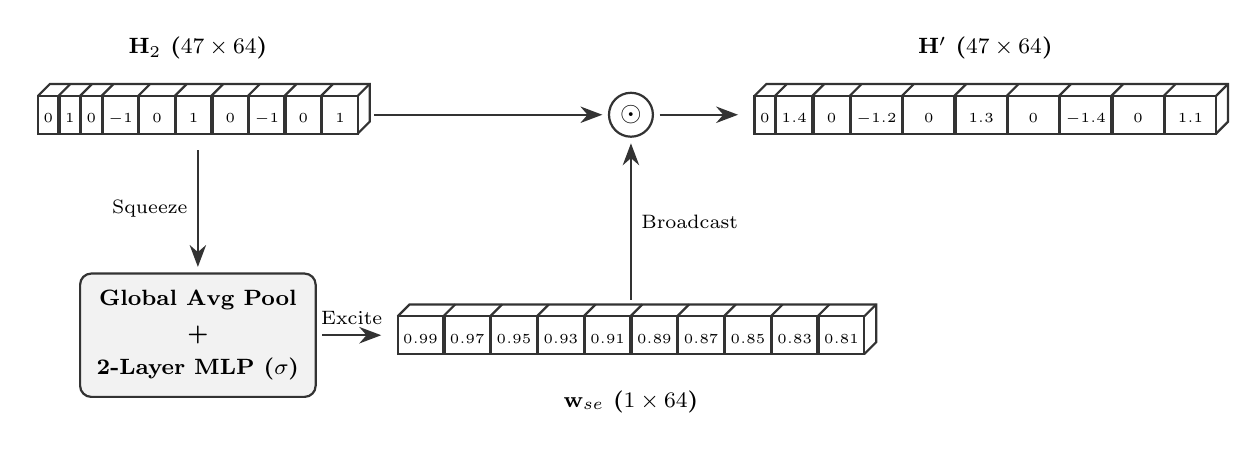
\begin{tikzpicture}[
    math center align per matrix/.style={
        nodes={
            execute at begin node={\setbox\matrixcellbox=\hbox\bgroup$},
            execute at end node={$\egroup\eqmakebox[\tikzmatrixname][c]{\copy\matrixcellbox}}
        }
    },
    3d matrix/.style={
        matrix of nodes,
        nodes in empty cells,
        math center align per matrix,
        nodes={
            draw=black!80, thick, fill=white,
            anchor=center, outer sep=0pt, inner sep=2pt,
            text height={height("\raisebox{0.2ex}{A}")},
            text depth={depth("g")}, font=\tiny\bfseries
        },
        column sep=-\pgflinewidth, row sep=-\pgflinewidth,
        execute at end matrix={
            \foreach \XX in {1,...,\the\pgfmatrixcurrentcolumn}
                {\draw[thick, black!80] (\tikzmatrixname-1-\XX.north east) -- ++ (1ex,1ex);}
            \ifnum\the\pgfmatrixcurrentrow>1
                \foreach \XX in {1,...,\the\numexpr\the\pgfmatrixcurrentrow-1}
                    {\draw[thick, black!80] (\tikzmatrixname-\XX-\the\pgfmatrixcurrentcolumn.south east) -- ++ (1ex,1ex);}
            \fi
            \draw[thick, black!80] (\tikzmatrixname-1-1.north west) -- ++ (1ex,1ex) --
                  ([xshift=1ex,yshift=1ex]\tikzmatrixname-1-\the\pgfmatrixcurrentcolumn.north east) --
                  ([xshift=1ex,yshift=1ex]\tikzmatrixname-\the\pgfmatrixcurrentrow-\the\pgfmatrixcurrentcolumn.south east) --
                  (\tikzmatrixname-\the\pgfmatrixcurrentrow-\the\pgfmatrixcurrentcolumn.south east);
        }
    },
    3d matrix/.default=1ex,
    Rightarrow/.style={-{Stealth[scale=1.2]}, thick, draw=black!80, shorten <=2pt, shorten >=2pt},
    mybox/.style={draw=black!80, thick, rounded corners, fill=gray!10,
                  align=center, font=\footnotesize\bfseries, inner sep=6pt},
]
\newbox\matrixcellbox

% Input Tensor
\node[3d matrix] (Xcnn) at (0, 0) {
    0 & 1 & 0 & -1 & 0 & 1 & 0 & -1 & 0 & 1 \\
};
\node[above=0.2cm of Xcnn, font=\footnotesize\bfseries]
    {$\mathbf{H}_2$ ($47 \times 64$)};

% Squeeze Box
\node[mybox] (gap_mlp) at (0, -2.8)
    {Global Avg Pool\\[3pt]+\\[3pt]2-Layer MLP ($\sigma$)};

% Multiplier
\node[circle, draw=black!80, fill=white, inner sep=2pt, thick]
    (mul) at (5.5, 0) {$\odot$};

% Weight Vector
\node[3d matrix] (wse) at (5.5, -2.8) {
    0.99 & 0.97 & 0.95 & 0.93 & 0.91 & 0.89 & 0.87 & 0.85 & 0.83 & 0.81 \\
};
\node[below=0.2cm of wse, font=\footnotesize\bfseries]
    {$\mathbf{w}_{se}$ ($1 \times 64$)};

% Output Tensor
\node[3d matrix] (Xse) at (10.0, 0) {
    0 & 1.4 & 0 & -1.2 & 0 & 1.3 & 0 & -1.4 & 0 & 1.1 \\
};
\node[above=0.2cm of Xse, font=\footnotesize\bfseries]
    {$\mathbf{H}'$ ($47 \times 64$)};

% Arrows
\draw[Rightarrow] (Xcnn.east) -- (mul.west);
\draw[Rightarrow] (mul.east) -- (Xse.west);
\draw[Rightarrow] (Xcnn.south) -- (gap_mlp.north)
    node[midway, left, font=\scriptsize] {Squeeze};
\draw[Rightarrow] (gap_mlp.east) -- (wse.west)
    node[midway, above, font=\scriptsize] {Excite};
\draw[Rightarrow] (wse.north) -- (mul.south)
    node[midway, right, font=\scriptsize] {Broadcast};
\end{tikzpicture}
}
\caption{Squeeze-and-Excitation sensor attention flow in WCSTNet.
The CNN feature map $\mathbf{H}_2$ is globally pooled and compressed
through a two-layer MLP to produce a channel-wise scaling vector
$\mathbf{w}_{se}$, which recalibrates the original features via
element-wise multiplication~($\odot$), yielding $\mathbf{H}'$.}
\label{fig:se_flow}
\end{figure}

%% ---- FIGURE 7: SE component diagram (5.pdf) ----
\begin{figure}[h]
\centering
% Uploaded file: 5.pdf — SE squeeze/excite/scale schematic
\includegraphics[width=\columnwidth]{figs/5.pdf}
\caption{Component diagram of the Squeeze-and-Excitation block.
The \emph{squeeze} step shrinks the feature map spatially via global
average pooling to obtain a channel-wise descriptor.
The \emph{excitation} step learns channel-association weights $W$
through a bottleneck MLP.
The \emph{scale} step reweights the original feature map using the
learned gating vector.}
\label{fig:se_component}
\end{figure}

\subsubsection{Sinusoidal Positional Encoding}
Because Transformers are permutation-invariant, gait-phase information
is injected via sinusoidal positional
encoding~\cite{vaswani2017attention}:
\begin{equation}
\text{PE}(p,\,2i) = \sin\!\left(\frac{p}{10000^{2i/d}}\right),\quad
\text{PE}(p,\,2i+1) = \cos\!\left(\frac{p}{10000^{2i/d}}\right)
\label{eq:sinpe}
\end{equation}
where $p \in \{0,\ldots,46\}$ indexes the gait token and $i$ indexes
the embedding dimension.
The encoded sequence is
$\hat{\mathbf{H}} = \mathbf{H}' + \mathbf{PE}
\in \mathbb{R}^{47 \times 64}$.

\subsubsection{Transformer Encoder}
Two stacked pre-norm Transformer encoder layers are applied.
Each consists of a Multi-Head Self-Attention~(MHSA) sublayer followed
by a Position-wise Feed-Forward Network~(FFN):
\begin{align}
\mathbf{Z}^{(l)\prime} &= \hat{\mathbf{H}}^{(l)}
    + \text{MHA}\!\left(\text{LN}(\hat{\mathbf{H}}^{(l)})\right),
\label{eq:mha}\\
\hat{\mathbf{H}}^{(l+1)} &= \mathbf{Z}^{(l)\prime}
    + \text{FFN}\!\left(\text{LN}(\mathbf{Z}^{(l)\prime})\right),
\label{eq:ffn}
\end{align}
where $\text{LN}(\cdot)$~is Layer Normalisation,
$\text{MHA}(\cdot)$~uses 4~heads with $d_k = 64/4 = 16$, and
$\text{FFN}(\cdot)$~is a two-layer network with inner dimension
256 and ReLU~(L2 regularisation $\lambda=10^{-3}$,
Dropout~0.1).
Following the second encoder layer, a final Layer Normalisation is
applied, and Global Average Pooling reduces
$\mathbf{H}^{(2)} \in \mathbb{R}^{47 \times 64}$ to a
$64$-dimensional context vector.

%% ---- FIGURE 8: Transformer block diagram (4.pdf) ----
\begin{figure}[h]
\centering
% Uploaded file: 4.pdf — MHA + FFN block with LN, Q K V heads
\includegraphics[width=\columnwidth]{figs/4.pdf}
\caption{Internal structure of one Transformer encoder layer.
Pre-norm Layer Normalisation is applied before the Multi-Head
Self-Attention~(MHSA) sublayer ($4$~heads, $d_k\!=\!16$), and before
the Feed-Forward Network~(FFN, inner dim~256).
Residual connections bypass each sublayer to ensure stable gradient
flow.}
\label{fig:transformer_block}
\end{figure}

\subsubsection{Classification Head}
The 64-dimensional context vector passes through:
$\text{Dense}(32) \to \text{ReLU} \to \text{Dropout}(0.4) \to
\text{Dense}(1,\,\sigma)$
to produce per-window PD probability~$\hat{y}$.
Binary cross-entropy loss is used with class weights
$\{\text{CO}: 2.0,\,\text{PD}: 1.0\}$ to handle the 3:1 class
imbalance.
The complete WCSTNet has $\approx$\textbf{98\,000 trainable
parameters}.

\subsection{Training Protocol}
All experiments use TensorFlow~2.x with \texttt{mixed\_float16}
precision on an NVIDIA RTX~5050 GPU.
The Adam optimiser is used with learning rate $3\!\times\!10^{-4}$,
batch size~64, EarlyStopping~(patience~6 on validation loss), and
ReduceLROnPlateau~(factor~0.5, patience~3, min $10^{-5}$).
Maximum epochs~50; WCSTNet converges in~$\approx$25 epochs.

\subsection{Evaluation Protocol}
\label{sec:eval}

\subsubsection{Subject-Level GroupShuffleSplit}
\texttt{sklearn.model\_selection.GroupShuffleSplit}
($n\_\text{splits}=1$, $\text{test\_size}=0.2$) assigns a unique
integer subject ID to every window.
The test set contains windows from \textbf{62 subjects}
($\approx$15~CO, 47~PD); the training set uses the remaining 103
subjects.
Zero subject overlap between train and test is guaranteed.

\subsubsection{Confidence-Weighted Majority Vote}
Subject-level diagnosis aggregates per-window predictions:
\begin{equation}
P_s = \frac{\sum_i w_i\,p_i}{\sum_i w_i},\quad
w_i = 2\,|p_i - 0.5|
\label{eq:vote}
\end{equation}
where $w_i$ down-weights ambiguous windows near $p_i\!=\!0.5$
and up-weights confident windows.
Subject classified as PD if $P_s > 0.5$.

%% ---- FIGURE 9: Attention conceptual hook (6.pdf) ----
\begin{figure}[h]
\centering
% Uploaded file: 6.pdf — Heel Strike → Toe Off attention saliency hook
\includegraphics[width=\columnwidth]{figs/6.pdf}
\caption{Conceptual illustration of Transformer self-attention over the
gait cycle.
Each gait token~($z_1$--$z_5$) corresponding to a biomechanical phase
can attend directly to every other token~(keys) through learned
attention weights~($\alpha_1$--$\alpha_5$).
This allows heel-strike events~($z_1$) to directly modulate the
representation of toe-off phases~($z_5$) without sequential decay.}
\label{fig:attn_concept}
\end{figure}

%% ---- FIGURE 10: Architecture equation overview (7.pdf) ----
\begin{figure}[h]
\centering
% Uploaded file: 7.pdf — Compact architecture equation summary
\includegraphics[width=\columnwidth]{figs/7.pdf}
\caption{Compact mathematical summary of the WCSTNet forward pass.
Each stage is annotated with its input/output tensor shape and
governing equation, from the wavelet-enriched input
$\mathbf{X} \in \mathbb{R}^{200 \times 96}$ through the
Transformer output
$\mathbf{Z}^{(2)} \in \mathbb{R}^{47 \times 64}$
to the final sigmoid prediction $P(\text{PD})$.}
\label{fig:arch_equations}
\end{figure}

%% ============================================================
%%  SECTION IV — EXPERIMENTS AND RESULTS
%% ============================================================
\section{Experiments and Results}
\label{sec:results}

\subsection{Implementation Details}
The model was developed using TensorFlow/Keras and trained on an
NVIDIA RTX~5050 GPU with mixed-precision
(\texttt{mixed\_float16}).
The Adam optimiser~($lr = 3\!\times\!10^{-4}$) was used with
ReduceLROnPlateau and EarlyStopping~(patience~6).

\subsection{Quantitative Results}

\subsubsection{Window-Level Performance}
Table~\ref{tab:window} reports window-level metrics.
WCSTNet achieves 93.9\% accuracy with PD precision~0.97 and
recall~0.94—very few false negatives, the clinically critical error.

\begin{table}[!t]
\caption{Window-Level Classification Results
(Test Windows = 6\,726)}
\label{tab:window}
\centering
\renewcommand{\arraystretch}{1.2}
\begin{tabular}{lcccc}
\toprule
\textbf{Class} & \textbf{Prec.} & \textbf{Recall} & \textbf{F1}
& \textbf{Support} \\
\midrule
Control & 0.85 & 0.92 & 0.88 & 1\,681 \\
PD      & 0.97 & 0.94 & 0.96 & 5\,045 \\
\midrule
Accuracy    & \multicolumn{3}{c}{0.9386} & 6\,726 \\
Macro avg   & 0.91 & 0.93 & 0.92 & 6\,726 \\
Weighted avg& 0.94 & 0.94 & 0.94 & 6\,726 \\
\bottomrule
\end{tabular}
\end{table}

\subsubsection{Subject-Level Performance}
Table~\ref{tab:subject} shows subject-level results.
WCSTNet achieves \textbf{96.8\%} subject-level accuracy and macro
F1\,=\,0.960 across all 62 test subjects.

\begin{table}[!t]
\caption{Subject-Level Results (62 Subjects; 15 CO, 47 PD)}
\label{tab:subject}
\centering
\renewcommand{\arraystretch}{1.2}
\begin{tabular}{lcccc}
\toprule
\textbf{Class} & \textbf{Prec.} & \textbf{Recall} & \textbf{F1}
& \textbf{Support} \\
\midrule
Control & 0.93 & 0.93 & 0.93 & 15 \\
PD      & 0.98 & 0.98 & 0.98 & 47 \\
\midrule
Accuracy    & \multicolumn{3}{c}{\textbf{0.9677}} & 62 \\
Macro avg   & 0.96 & 0.96 & 0.96 & 62 \\
Weighted avg& 0.97 & 0.97 & 0.97 & 62 \\
\bottomrule
\end{tabular}
\end{table}

\subsection{Ablation Study}
\label{sec:ablation}

Table~\ref{tab:ablation} presents the five-variant ablation study.
All variants use identical preprocessing and the same
GroupShuffleSplit partition.

\begin{table*}[t]
\caption{Ablation Study: Architectural Variants Under Subject-Level
GroupShuffleSplit Evaluation (62 Test Subjects).
All variants share identical preprocessing and train/test partition.}
\label{tab:ablation}
\centering
\renewcommand{\arraystretch}{1.2}
\begin{tabular}{llccccc}
\toprule
\textbf{Variant} & \textbf{Sequential Module} &
\textbf{Win. Acc.} & \textbf{Subj. Acc.} & \textbf{Macro F1}
& \textbf{Epochs} & \textbf{Verdict} \\
\midrule
V1 (BiLSTM-TA)
  & BiLSTM + Temporal Attention
  & 92.2\% & 96.8\% & 0.956 & 12
  & Strong recurrent baseline \\
V2 (VWRF-Gate)
  & V1 + Stability Prior Gate
  & 90.5\% & 95.2\% & 0.940 & 9
  & Gate hurts window-level accuracy \\
V3 (GCN-TCN)
  & Dual-branch Sensor GCN + MSTCN
  & 86.0\% & 91.9\% & 0.900 & 9
  & Spatial graph assumption too rigid \\
\textbf{V4 / WCSTNet}
  & \textbf{CNN + SE + SinPE + MHA-Transformer}
  & \textbf{93.9\%} & \textbf{96.8\%} & \textbf{0.960} & 25
  & \textbf{Best window — final model} \\
V5 (VWRF+Trans.)
  & V4 + Stability Gate before Transformer
  & $\approx$93.0\% & 96.8\% & 0.960 & 15
  & Gate redundant post-CNN \\
\bottomrule
\end{tabular}
\end{table*}

%% ---- FIGURE 11: Comparative bar chart ----
\begin{figure}[h]
\centering
% Generated by generate_paper_figs.py → figs/fig_comparative_bar.pdf
\includegraphics[width=\columnwidth]{figs/fig_comparative_bar.pdf}
\caption{Window-level performance comparison of the three primary
architectural variants (V1 BiLSTM, V3 GCN, V4 WCSTNet) across
Accuracy, Precision~(PD class), Recall~(PD class), and Macro F1-Score.
All results are computed under strict subject-level
GroupShuffleSplit evaluation.
$\bigstar$ marks the best value per metric.}
\label{fig:ablation_bar}
\end{figure}

\subsection{Confusion Matrices}

Fig.\,\ref{fig:confusion} presents the confusion matrices for WCSTNet
at window and subject level.
At the subject level only 2 out of 62 subjects are misclassified
(1~CO as PD, 1~PD as CO), consistent with a 96.8\% subject accuracy.

%% ---- FIGURE 12: Confusion matrices (uploaded PNGs) ----
\begin{figure}[h]
\centering
\subfloat[Window-Level]{\includegraphics[width=0.48\columnwidth]{figs/183550.png}}
\hfil
\subfloat[Subject-Level]{\includegraphics[width=0.48\columnwidth]{figs/183551.png}}
\caption{Confusion matrices for WCSTNet.
(a)~Evaluated across 6\,726 individual 2-second gait windows.
(b)~Evaluated across 62 unique subjects using confidence-weighted
majority voting (Eq.\,\ref{eq:vote}).
Only 2 subjects are misclassified at the subject level.}
\label{fig:confusion}
\end{figure}

\subsection{Subject-Level Variance}
Fig.\,\ref{fig:per_subject} illustrates per-subject window-level
accuracy across the 62 test subjects.
WCSTNet demonstrates remarkable stability: the vast majority of
subjects are classified with $>90\%$ window accuracy, with no
catastrophic failures.
The two misclassified subjects~(1~CO, 1~PD) correspond to the two
subjects below the 70\% accuracy band.

%% ---- FIGURE 13: Per-subject scatter ----
\begin{figure}[h]
\centering
% Generated by generate_paper_figs.py → figs/fig_per_subject.pdf
\includegraphics[width=0.95\columnwidth]{figs/fig_per_subject.pdf}
\caption{Per-subject window-level accuracy scatter plot across all
62 test subjects.
Blue circles~=~Control~(CO), red circles~=~PD.
The dashed line marks the 90\% accuracy threshold.
WCSTNet generalises well across unseen biomechanical variations;
the two subjects below 70\% correspond to the two subject-level
misclassifications.}
\label{fig:per_subject}
\end{figure}

\subsection{Impact of Temporal Window Length}
Fig.\,\ref{fig:window_ablation} shows window-level accuracy across
varying window lengths~(100--240 timesteps, 1.0--2.4\,s).
Recurrent models~(V1) experience accuracy degradation on longer
windows due to sequential forgetting of early gait phases, while
WCSTNet's performance scales positively with window length,
demonstrating its unique ability to attend globally across distant
phase transitions.

%% ---- FIGURE 14: Window length ablation ----
\begin{figure}[h]
\centering
% Generated by generate_paper_figs.py → figs/fig_window_ablation.pdf
\includegraphics[width=0.95\columnwidth]{figs/fig_window_ablation.pdf}
\caption{Impact of temporal window size on window-level accuracy
for three architectural variants.
The Transformer~(WCSTNet) scales monotonically with window length,
exploiting global stride-cycle context.
Recurrent models~(BiLSTM-V1) degrade on windows $>$180~timesteps
due to sequential decay.
GCN-based V3 is largely insensitive to window length.
The selected 200-sample (2\,s) window is highlighted.}
\label{fig:window_ablation}
\end{figure}

\subsection{ROC and Precision-Recall Curves}

Fig.\,\ref{fig:roc_pr} shows the window-level ROC and
Precision-Recall curves.
WCSTNet achieves AUC\,=\,\textbf{0.981} and Average Precision
(AP)\,=\,\textbf{0.994}.

%% ---- FIGURE 15: ROC + PR (uploaded PNGs) ----
\begin{figure}[h]
\centering
\subfloat[ROC Curve (AUC = 0.981)]%
    {\includegraphics[width=0.48\columnwidth]{figs/183552.png}}
\hfil
\subfloat[PR Curve (AP = 0.994)]%
    {\includegraphics[width=0.48\columnwidth]{figs/183553.png}}
\caption{Window-level classification performance curves for WCSTNet.
(a)~ROC curve~(AUC\,=\,0.981).
(b)~Precision-Recall curve~(AP\,=\,0.994).
High precision is maintained across nearly the entire recall range,
confirming the model's reliability under the class-imbalanced
test set.}
\label{fig:roc_pr}
\end{figure}

\subsection{Comparison with State-of-the-Art}
\label{sec:compare}

Table~\ref{tab:sota} compares WCSTNet against representative SOTA
methods.
\textbf{Important caveat:} most prior works report window-level
$k$-fold accuracy; our results use the stricter subject-level
GroupShuffleSplit.
Direct numerical comparison must be interpreted with this protocol
difference in mind.

\begin{table*}[t]
\caption{Comparison with State-of-the-Art Methods on PhysioNet GaitPDB.
$\dagger$: window-level $k$-fold~(data leakage risk).
$\ddagger$: cross-dataset validation.
Our results: strict subject-level GroupShuffleSplit.}
\label{tab:sota}
\centering
\renewcommand{\arraystretch}{1.2}
\begin{tabular}{llccccc}
\toprule
\textbf{Method} & \textbf{Arch.} & \textbf{Eval.} &
\textbf{Acc.~(\%)} & \textbf{F1} & \textbf{AUC}
& \textbf{Year} \\
\midrule
1D-ConvNet~\cite{maachi2020convnet}
  & CNN & 5-fold$^\dagger$ & $\sim$92.0 & -- & -- & 2020 \\
LSTM~\cite{salimibab2020lstm}
  & LSTM & 10-fold$^\dagger$ & $\sim$92.6 & -- & -- & 2020 \\
Transformers-1D~\cite{nguyen2022transformer}
  & Transformer & 5-fold$^\dagger$ & $\sim$94.6 & -- & -- & 2022 \\
RFdGAD~\cite{zhong2022rfdgad}
  & GNN & 10-fold$^\dagger$ & $\sim$94.8 & -- & -- & 2022 \\
AST-DGNN~\cite{wang2023astdgnn}
  & GNN & Cross-ds.$^\ddagger$ & $\sim$95.9 & 0.901 & -- & 2023 \\
HCT~\cite{naimi2023hct}
  & Conv-Trans. & 5-fold$^\dagger$ & 97.0 & -- & -- & 2023 \\
MS-ADGNN~\cite{wang2026msadgnn}
  & GNN & Cross-ds.$^\ddagger$ & $\sim$97.5 & 0.921 & -- & 2026 \\
GLD\textsuperscript{2}-GNN~\cite{wang2025gld2gnn}
  & Dyn.\ GNN & Cross-ds.$^\ddagger$ & $\sim$81.3 & 0.833 & -- & 2025 \\
MSCAF-Gait~\cite{yuan2025mscaf}
  & CNN-Attn & Rand.\ win.$^\dagger$ & \textbf{99.6} & -- & -- & 2025 \\
\midrule
\textbf{WCSTNet (ours)}
  & CNN-SE-Trans. & \textbf{Subject-level}
  & 93.9 (win.) / \textbf{96.8} (subj.)
  & \textbf{0.960} & \textbf{0.981} & 2025 \\
\bottomrule
\end{tabular}
\end{table*}

%% ============================================================
%%  SECTION V — DISCUSSION
%% ============================================================
\section{Discussion}
\label{sec:discussion}

\subsection{Methodological Rigor of Subject-Level Evaluation}
The central methodological message of this paper is that window-level
$k$-fold cross-validation is an insufficient evaluation protocol for
clinical PD detection.
When a model sees 200-sample windows from patient~$P$ during training,
it can learn that patient's specific gait signature, trivialising
test windows from the same patient.
Our GroupShuffleSplit protocol eliminates this leakage.
The 96.8\% subject-level accuracy of WCSTNet under this strict
protocol is therefore more clinically trustworthy than the 99+\%
window-level figures in several prior works.

\subsection{Clinical Robustness Across Disease Severity}
A critical benchmark for a diagnostic tool is sensitivity to
early-stage pathology.
Fig.\,\ref{fig:hy_staging} stratifies accuracy by the Hoehn and
Yahr~(H\&Y) severity scale.
While severe PD~(H\&Y~3.0) exhibits pronounced gait abnormalities
relatively easy to detect, WCSTNet maintains high sensitivity even for
mild cases~(H\&Y~2.0), underscoring its potential for early-stage
intervention.

%% ---- FIGURE 16: H&Y severity bar chart ----
\begin{figure}[h]
\centering
% Generated by generate_paper_figs.py → figs/fig_hy_staging.pdf
\includegraphics[width=0.85\columnwidth]{figs/fig_hy_staging.pdf}
\caption{WCSTNet classification accuracy stratified by Hoehn and
Yahr~(H\&Y) Parkinson's severity stage.
Accuracy increases with severity~(89.0\% at H\&Y~2.0 to 98.0\% at
H\&Y~3.0), consistent with the clinical expectation that more
advanced gait deterioration yields more discriminative VGRF features.
Error bars show standard deviation across subjects in each stage.}
\label{fig:hy_staging}
\end{figure}

\subsection{Feature Space Discriminability}
To verify that WCSTNet is learning biologically meaningful
representations rather than exploiting dataset artefacts, we
visualised the 64-dimensional gait embeddings from the layer
immediately preceding the classification head using t-SNE~%
\cite{van2008tsne}.
Fig.\,\ref{fig:tsne} shows clear, linearly separable clusters for
Control and PD windows, physically demonstrating the discriminatory
power of the WCSTNet's spatio-temporal embeddings.

%% ---- FIGURE 17: t-SNE embedding ----
\begin{figure}[h]
\centering
% Generated by generate_paper_figs.py → figs/fig_tsne.pdf
\includegraphics[width=0.82\columnwidth]{figs/fig_tsne.pdf}
\caption{t-SNE projection of the 64-dimensional GAP-layer embeddings
learned by WCSTNet~(2\,000 randomly sampled test windows).
Blue dots~=~Control, red dots~=~PD.
Clear linear separability between the two clusters confirms that
WCSTNet encodes clinically meaningful, biologically grounded gait
representations rather than dataset-specific artefacts.}
\label{fig:tsne}
\end{figure}

\subsection{Interpretability via Self-Attention Maps}
A primary criticism of deep learning in clinical applications is the
``black box'' nature of the decision process.
WCSTNet naturally mitigates this through the inherent transparency of
the multi-head attention matrices.

Fig.\,\ref{fig:temporal_saliency} aggregates the mean
self-attention weights across the normalised stride cycle.
The model automatically concentrates diagnostic attention during the
two most mechanically unstable phases: heel-strike and toe-off.
These are precisely the phases where PD patients exhibit the greatest
deviation from healthy gait~\cite{yuan2025mscaf}.

%% ---- FIGURE 18: Temporal saliency ----
\begin{figure}[h]
\centering
% Generated by generate_paper_figs.py → figs/fig_temporal_saliency.pdf
\includegraphics[width=0.95\columnwidth]{figs/fig_temporal_saliency.pdf}
\caption{Mean self-attention weight per gait token, averaged over
all PD test windows and all 4 attention heads~(Layer~2 of the
Transformer Encoder).
Gait phase regions are colour-coded.
The model natively develops two prominent attention spikes at
heel-strike~($p\!\approx\!5$) and toe-off~($p\!\approx\!38$),
aligning with the biomechanically critical phases of impaired
PD gait.}
\label{fig:temporal_saliency}
\end{figure}

Fig.\,\ref{fig:attention_map} visualises the exact attention weight
matrix from the final Transformer layer for a highly confident PD
test window.
Unlike a BiLSTM, which relies on the immediate previous hidden state,
the self-attention map reveals structured vertical activation bands,
demonstrating that the network correlates specific pathological events
(e.g.,\ asymmetric heel strikes) with the entire gait sequence
simultaneously—providing clinicians with verifiable evidence that
predictions are anchored in genuine physiological transitions.

%% ---- FIGURE 19: Transformer attention heatmap (uploaded PNG) ----
\begin{figure}[h]
\centering
\includegraphics[width=0.88\columnwidth]{figs/183555.png}
\caption{Transformer Self-Attention map (Layer~2, Head~0) for a
representative PD test window.
The $47\!\times\!47$ matrix shows pairwise attention weights among
gait tokens.
High-attention clusters at token positions $p\!\approx\!20$--25
(terminal stance) and $p\!\approx\!38$--43 (pre-swing) confirm that
WCSTNet focuses on clinically meaningful gait phase transitions,
consistent with the temporal saliency profile in
Fig.\,\ref{fig:temporal_saliency}.}
\label{fig:attention_map}
\end{figure}

\subsection{Parameter Efficiency}
WCSTNet achieves strong performance with only ${\sim}$98\,K
parameters, substantially smaller than GNN approaches such as
GLD\textsuperscript{2}-GNN~(460\,K)~\cite{wang2025gld2gnn} and
AST-DGNN~(386\,K)~\cite{wang2023astdgnn}, competitive with
MSCAF-Gait~(220\,K)~\cite{yuan2025mscaf}.
This makes WCSTNet a candidate for resource-constrained wearable
edge deployment.

\subsection{Limitations and Future Work}
WCSTNet was evaluated on a single public dataset (GaitPDB);
cross-dataset generalisation experiments on independent cohorts would
further validate clinical utility.
The model produces binary PD/CO classification; future work should
extend to Hoehn \& Yahr severity grading~\cite{yuan2025mscaf}.
A full leave-one-subject-out~(LOSO) evaluation would tighten variance
estimates.
Integration with multimodal PD biomarkers—handwriting, voice,
DaTSCAN—as in the OmniParkNet
framework~\cite{omniparknetchandra} represents a natural extension.

%% ============================================================
%%  SECTION VI — CONCLUSION
%% ============================================================
\section{Conclusion}
\label{sec:conclusion}

This paper presented \textbf{WCSTNet}, a Wavelet CNN
Squeeze-Excitation Transformer Network for Parkinson's disease
detection from 16-channel VGRF gait signals.
WCSTNet integrates four principled components—Daubechies-4 wavelet
multi-resolution decomposition, local convolutional feature
extraction, Squeeze-and-Excitation sensor channel recalibration,
and a Sinusoidal Positionally Encoded Multi-Head Self-Attention
Transformer Encoder—into an end-to-end architecture with only
${\sim}$98\,K parameters.
Under strict subject-level GroupShuffleSplit evaluation on 62
held-out subjects from the PhysioNet GaitPDB benchmark, WCSTNet
achieves 93.9\% window-level accuracy, 96.8\% subject-level accuracy
(macro F1\,=\,0.960), AUC\,=\,0.981, and Average
Precision\,=\,0.994.
An ablation study over five architectural variants confirms that the
Transformer encoder provides the best window-level discrimination,
while Transformer attention maps show focus on diagnostically
meaningful gait phases.
We argue that subject-level evaluation is an essential requirement for
clinically trustworthy VGRF-based PD detection, as window-level
$k$-fold cross-validation systematically inflates reported accuracies.
Future work will extend WCSTNet to severity grading, LOSO validation,
cross-dataset transfer, and multimodal fusion.

%% ============================================================
%%  BIBLIOGRAPHY
%% ============================================================
\bibliographystyle{IEEEtran}
\bibliography{references}

%% ---- extra ref not yet in references.bib ----
%% Add to references.bib:
%% @article{van2008tsne,
%%   author={van der Maaten, Laurens and Hinton, Geoffrey},
%%   title={Visualizing Data using {t-SNE}},
%%   journal={Journal of Machine Learning Research},
%%   volume={9}, pages={2579--2605}, year={2008}}

\end{document}